% ====== TAREA 2 MATEMATICAS APLICADAS ======
\documentclass{article}
\usepackage[utf8]{inputenc}
\usepackage[spanish]{babel}
\usepackage{amsmath, amsfonts, amssymb}
\usepackage{graphicx}
\usepackage[usenames]{color}
\usepackage[text={20cm,25cm},centering,top=1.5cm,bottom=1.5cm,letterpaper,showframe=false]{geometry}
\renewcommand{\baselinestretch}{1.5}
\parindent  = 0mm
\parskip    = 4mm
\definecolor{azul}{RGB}{10,80,190}
\definecolor{negro}{RGB}{0,0,0}
\definecolor{rojo}{RGB}{190,80,10}
\definecolor{verde}{RGB}{0,120,50}

\begin{document}
    \title{Tarea 2}
    \author{Careaga Carrillo Juan Manuel\\
            Quiróz Castañeda Edgar\\
            Soto Corderi Sandra del Mar}
    \date{Miércoles 10 de octubre de 2018}
    \maketitle
    \begin{enumerate}

        % Ejercicio 1
        \item {
            Encontrar la imagen de un triángulo con vértices $(0,0)$, $(1,1)$
            y $(0,1)$ bajo la transformación $x=u^2$ y $y=v$.

            \color{azul}
            Despejando $u$ de $x=u^2$, tenemos que $u=\sqrt{x}$ y que $v = y$\\
            De ahí, tendríamos que la transformación es:\\
            $T(x,y) = (\sqrt{x} , y)$

           	Aplicamos la transformación a sus vértices\\
            $T(0,0) = (\sqrt{0}, 0) = (0,0)$\\
            $T(1,1) = (\sqrt{1}, 1) = (1,1)$\\
            $T(0,1) = (\sqrt{0}, 1) = (0,1)$

            Por lo tanto, la imagen del triángulo es el mismo triángulo antes
            de ser transformado
            \begin{center}
                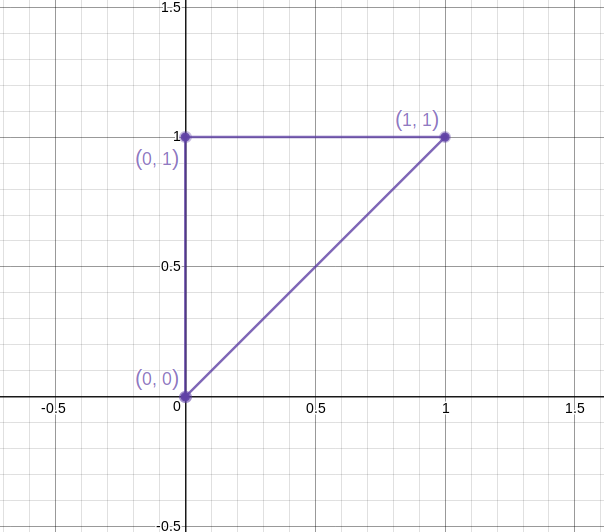
\includegraphics[width=6cm]{img/ejercicio1.png}
                \hspace{.5cm}
                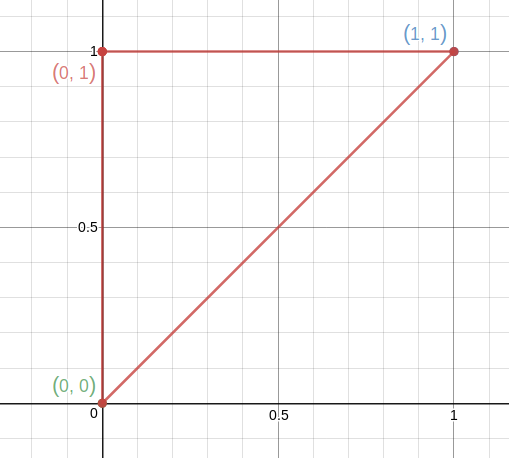
\includegraphics[width=6cm]{img/ejercicio1-1.png}
        	\end{center}
            En la imagen izquierda vemos el triángulo original, y en la derecha
            vemos la imagen del triángulo bajo la transformación.
	    }

        % Ejercicio 2
        \item {
            Calcular
            \[
                \iint_{D}{e^{\frac{x-2y}{3x-y}}\,dA}
            \]
            con $D$ el paralelogramo acotado por las rectas $x-2y=0$, $x-2y=$,
            $3x-y=1$ y $3x-y=8$-

            \color{azul}
        %     El paralelogramo $D$ lo podemos ver como la siguiente imagen:\\
        %     \begin{center}
        %         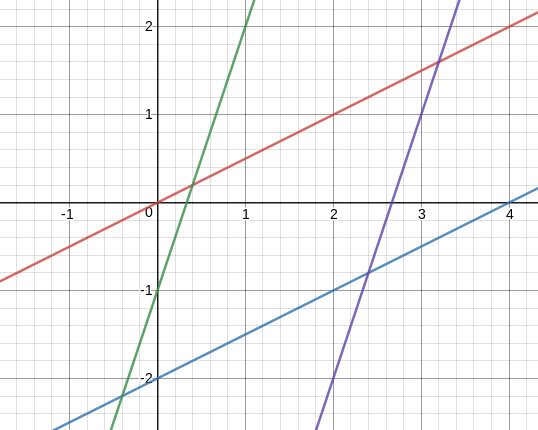
\includegraphics[width=8cm]{img/ejercicio2.png}
        % 	\end{center}

        %     Para facilitar la integral, ralizaremos un cambio de variable y una
        %     transformación lineal con D.\\
        %     Obtenemos el Jacobiano de la siguiente forma:
        %     \[
        %         \begin{bmatrix}
        %             \frac{\partial x}{\partial u}&
        %             \frac{\partial x}{\partial v}\\
        %             \frac{\partial y}{\partial u}&
        %             \frac{\partial y}{\partial v}\\
        %         \end{bmatrix}
        %         =
        %         \begin{bmatrix}
        %             -\frac{1}{5}
        %             &\frac{2}{5}\\
        %             -\frac{3}{5}
        %             &\frac{1}{5}\\
        %         \end{bmatrix}
        %         =-\frac{7}{25}
        %     \]
        %     Para la transformación, tomamos $u = x-2y$ y $v= 3x-y$.
            
        %     Despejando con un sistema de ecuaciones de u y v, tenemos que
        %     $x = -(\frac{u-2v}{5})$ y  $y = -(\frac{3u-v}{5})$

        %     De ahí, si aplicamos la transformación en los lados del
        %     paralelogramo tenemos:
        %     $$T(x-2y=0) \Rightarrow (\frac{-u+2v}{5}) + 2(\frac{3u-v}{5}) =
        %     \frac{-u+2v+6u-2v}{5} = \frac{5u}{5} \Rightarrow u = 0$$
        %     $$T(x-2y=4) \Rightarrow (\frac{-u+2v}{5}) + 2(\frac{3u-v}{5}) =
        %     \frac{-u+2v+6u-2v}{5} = \frac{5u}{5} \Rightarrow u = 4$$
        %     $$T(3x-y=1) \Rightarrow -3(\frac{u-2v}{5}) + (\frac{3u-v}{5}) =
        %     \frac{-3u+6v+3u-v}{5} = \frac{5v}{5} \Rightarrow v = 1$$
        %     $$T(3x-y=8) \Rightarrow -3(\frac{u-2v}{5}) + (\frac{3u-v}{5}) =
        %     \frac{-3u+6v+3u-v}{5} = \frac{5v}{5} \Rightarrow v = 8$$

        % 	La imagen del paralelogramo bajo la transformación es como la siguiente imagen, vemos que es un cuadrado, así que los límites de u y v son sencillos.
        %     \begin{center}
        %         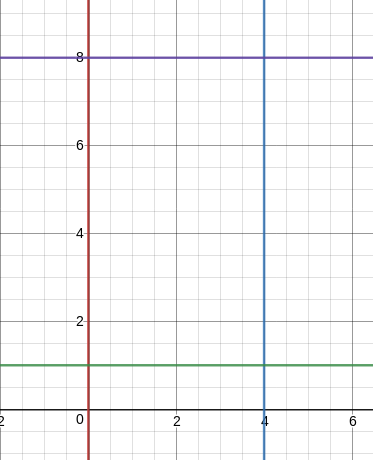
\includegraphics[width=6cm]{img/ejercicio2-1.png}
        % 	\end{center}
        %     De ahí, podemos resolver a nuestra integral doble como:

        %     $$\int_{1}^{8}\int_{0}^{4}-\frac{7}{25}e^{\frac{u}{v}}\,du\,dv$$
            
        %     (Usando integración por sustitución tomando $s =\frac{u}{v}$,
        %     resolvemos directamente $du$) Tenemos:

        %     $$= -\frac{7}{25} \int_{1}^{8} v(e^{\frac{4}{v}} -1)dv$$

        %     $$\int_{1}^{8} v(e^{\frac{4}{v}} -1)dv = \int_{1}^{8}
        %     ve^{\frac{4}{v}}dv - \int_{1}^{8} vdv$$

        %     $$\int_{1}^{8} vdv = \frac{v^2}{2}\Big|_1^8 = \frac{63}{2}$$
            
        %     (Usando integración por sustitución tomando $t =\frac{4}{v}$,$dt = -\frac{v^2}{4}dv$ y $v= \frac{4}{t}$) Tenemos:
        %     $$\int_{1}^{8} ve^{\frac{4}{v}}dv = -16\int_{1}^{8} \frac{e^{t}}{t^3}dt$$
        %     (Usando integración por partes donde $u = e^t$ y $dv = \frac{1}{t^3}$)
        %     $\int_{1}^{8} \frac{e^{t}}{t^3}dt = -\frac{e^t}{2t^2} + \int-\frac{e^t}{2t^2}dt$\\
        %     (Usando integración por partes donde $u = e^t$ y $dv = \frac{1}{2t^2})$)\\
        %     $\int-\frac{e^t}{2t^2} = -\frac{1}{2} (-\frac{e^t}{t} + \int\frac{e^t}{t}dt)$\\
        %     (Usando la definición $Ei(t) = \int\frac{e^t}{t}dt$, resolvemos el resto de integral. También regresamos a los valores originales)\\
        %     $\int_{1}^{8} ve^{\frac{4}{v}}dv = [-16(-\frac{1}{32}e^{\frac{4}{v}}v^2 + \frac{1}{2}(-\frac{1}{4})e^{\frac{4}{v}}v + Ei(\frac{4}{v}))]\Big|_1^8$\\

        %     De todo lo anterior, el resultado sería:\\
        %     $\int_{1}^{8}\int_{0}^{4}-\frac{7}{25}e^{\frac{u}{v}}dudv = (-\frac{7}{25})(48\sqrt{e} - 8Ei(\frac{1}{2}) - 32 - \frac{5e^4 - 16Ei(4)}{2})$
        }

        % Ejercicio 3
        \item {
            Hallar el volumen del elipsoide
            \[
                \frac{x^2}{a^2}+\frac{y^2}{b^2}+\frac{z^2}{c^2}\leq 1
            \]

            \color{azul}
            Hallar el volumen de forma típica nos daría una integral triple
            bastante compleja, así que para auxiliarnos, transformamos la
            elipsoide a coordenas esféricas y realizamos un cambio de variables.
            \begin{center}
                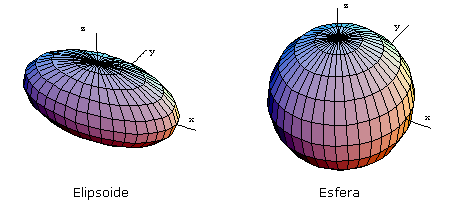
\includegraphics[width=10cm]{img/elipsoide.png}
        	\end{center}
            Tomamos las coordenadas esféricas:
            \begin{align*}
                x &= ar\sen\gamma\cos{\theta}\\
                y &= br\sen\gamma\sen{\theta}\\
                x &= cr\cos\gamma
            \end{align*}

            El jacobiano sería la multiplicación de $abc$ con el jacobiano de
            coordenadas esféricas que vimos en clase es $r^2\sin\gamma$. De ahí,
            el jacobiano es $abcr^2\sin\gamma$

            El elipsoide es simétrico respecto al origen, los ejes y los planos
            de coordenadas. Además las secciones con planos paralelos a los
            coordenados son elipses (caso particular: circunferencia). De esta
            forma si vemos al elipsoide en coordenas esféricas podemos
            representar su volumen de esta manera:
        	\[
                \int_{0}^{1}{
                    \int_{0}^{2\pi}{
                        \int_{0}^{\pi}{
                            abcr^2\sen\gamma
                        \,d\gamma}
                    \,d\theta}
                \,dr}
            \]
            Debido a que las variables son independientes una de otra podemos
            resolver la integral así:
            \[
                (abc)
                \left(\int_{0}^{1}r^2 dr\right)
                \left(\int_{0}^{2\pi} d\theta\right)
                \left(\int_{0}^{\pi}\sin\gamma d\gamma\right)
                =
                (abc)
                \left(\frac{r^3}{3}\Big|_0^1\right)
                \left(\theta\Big|_0^{2\pi}\right)
                \left(-\cos{\gamma}\Big|_0^{\pi}\right)
                =
                (abc)\left(\frac{1}{3}\right)
                \left(2\pi\right)(2)
                =
                \frac{4}{3}\pi abc
            \]
            Por lo tanto, el volumen del elipsoide es
            $\displaystyle \frac{4}{3}\pi abc$.
        }

        % Ejercicio 4
        \item {
            Hallar el área acotada por la lemniscata
            \(
                \left(x^2+y^2\right)^2=2a^2\left(x^2-y^2\right)
            \).

            \color{azul}
            % Respuesta
        }

        % Ejercicio 5
        \item {
            Evaluar la integral iterada
            \[
                \int_{0}^{2}{
                    \int_{-\sqrt{2x-x^2}}^{\sqrt{2x-x^2}}{
                        \int_{0}^{x^2+y^2}{
                            \sqrt{x^2+y^2}
                        \,dz}
                    \,dy}
                \,dx}
            \]
            y bosquejar la región de integración $W$.

            \color{azul}
            % Respuesta
        }

        % Ejercicio 6
        \item {
            Calcular la masa del sólido que se encuentra fuera de la esfera
            $x^2+y^2+^z2=1$ y dentro de la esfera $x^2+y^2+z^2=2$ suponiendo
            que la densidad en un punto $P$ es directamente proporcional al
            cuadrado de la distancia de $P$ al centro de la esfera.

            \color{azul}
            % Respuesta
        }

        % Ejercicio 7
        \item {
            Determinar los números reales $\lambda$ para los que
            \[
                \iint_D {\frac{dA}{\left(x^2+y^2\right)^\lambda}}
            \]
            es convergente, con $D$ el disco unitario con centro en el origen.

            \color{azul}
            % Respuesta
            \begin{center}
                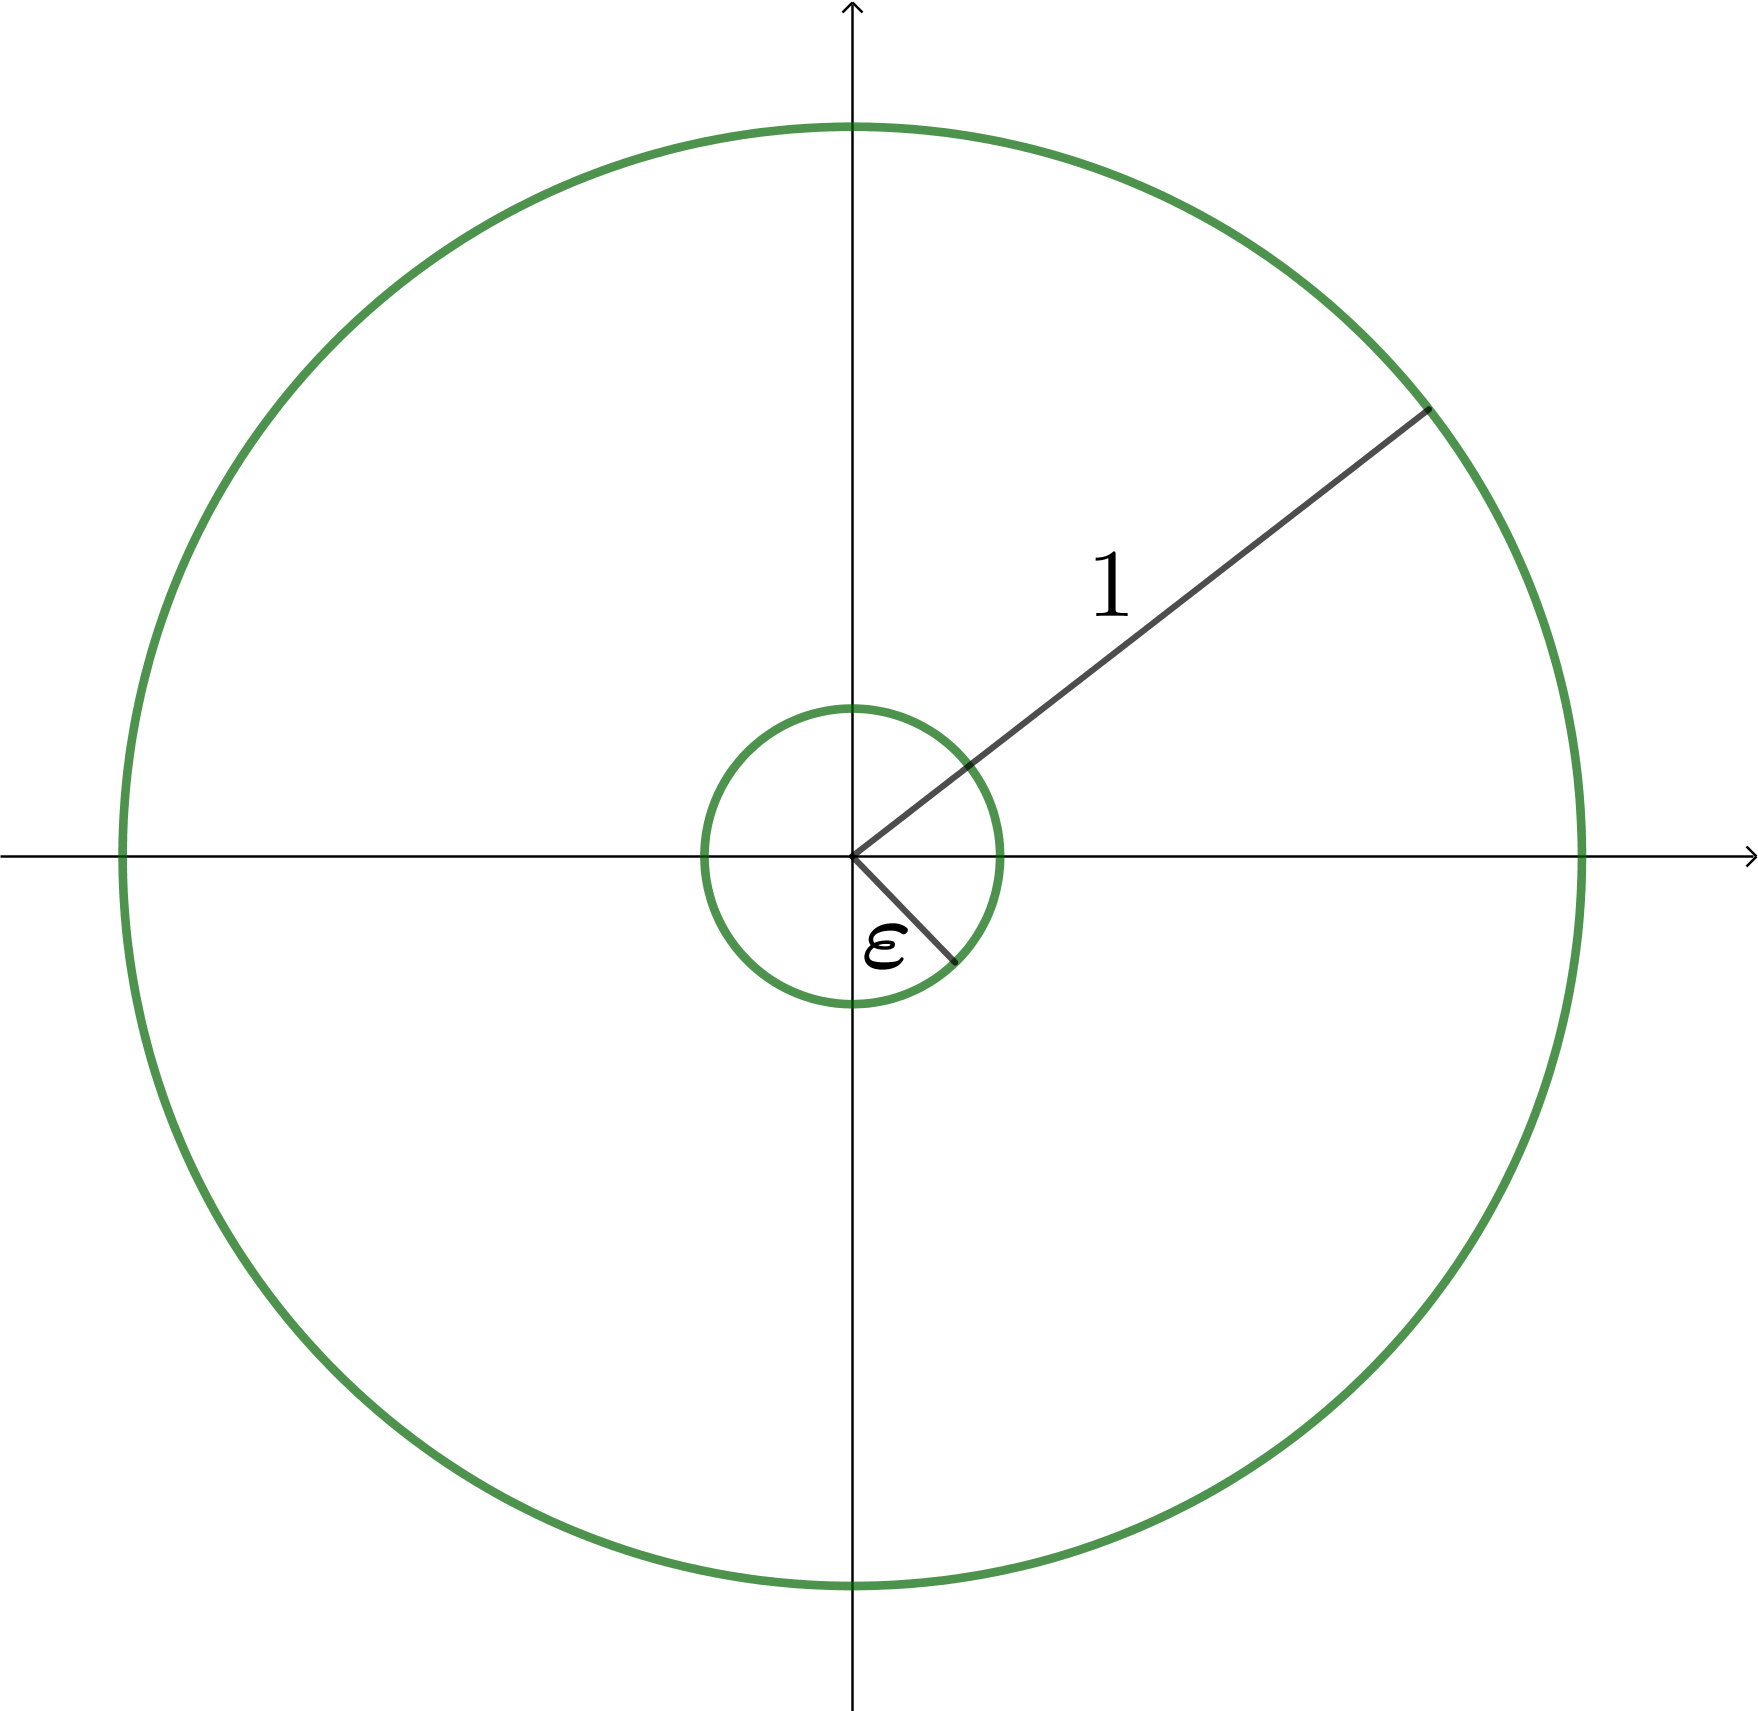
\includegraphics[width=4cm]{img/ej7.png}
            \end{center}
            La función $\displaystyle f(x)=\frac{1}{(x^2+y^2)^\lambda}$ no está
            definida cuando $x^2+y^2=0$, así que definimos una nueva región de
            integración $D_\varepsilon = \left\{(x,y)\in\mathbb{R}^2 |
            \varepsilon\leq x^2+y^2\leq 1\right\}$ y hacemos $\varepsilon
            \to 0$
            \[
                \iint_D {\frac{dA}{\left(x^2+y^2\right)^\lambda}}
                =\lim_{\varepsilon\to 0}{
                    \iint_{D_\varepsilon}{
                        \frac{dA}{\left(x^2+y^2\right)^\lambda}
                    }
                }
            \]
            para resolver la integral, conviene hacer una transformación a
            coordenadas polares
            \[
                \iint_D {\frac{dA}{\left(x^2+y^2\right)^\lambda}}
                =\int_{0}^{2\pi}{
                    \int_{0}^{1}{
                        \frac{r}{r^{2\lambda}}
                    \,dr}
                \,d\theta}
                =\lim_{\varepsilon\to 0}{
                    \int_{0}^{2\pi}{
                        \int_{\varepsilon}^{1}{
                            r^{1-2\lambda}
                        \,dr}
                    \,d\theta}
                }
            \]
            resolviendo la integral iterada (considerando $\lambda \ne 1$)
            \begin{align*}
                \lim_{\varepsilon\to 0}{
                    \int_{0}^{2\pi}{
                        \int_{\varepsilon}^{1}{
                            r^{1-2\lambda}
                        \,dr}
                    \,d\theta}
                }
                &=\lim_{\varepsilon\to 0}{
                    \int_{0}^{2\pi}{
                        \left[
                            \frac{r^{2-2\lambda}}
                                 {2-2\lambda}
                        \right]_{\varepsilon}^{1}
                    \,d\theta}
                }\\[.2cm]
                &=\lim_{\varepsilon\to 0}{
                    \int_{0}^{2\pi}{
                        \frac{1-\varepsilon^{2(1-\lambda)}}
                             {2(1-\lambda)}
                    \,d\theta}
                }\\[.2cm]
                &=\lim_{\varepsilon\to 0}{
                    \frac{2\pi[1-\varepsilon^{2(1-\lambda)}]}
                         {2(1-\lambda)}
                }\\[.2cm]
                &=\lim_{\varepsilon\to 0}{
                    \frac{\pi[1-\varepsilon^{2(1-\lambda)}]}
                         {1-\lambda}
                }
            \end{align*}
            Haciendo un análisis de ésta última expresión, concluimos que:
            \begin{itemize}
                \item si $\lambda>1$, entonces $1-\lambda>0$ y
                    $\varepsilon^{2(1-\lambda)}\to\infty$ (diverge)
                \item es cuando $\lambda<1$, entonces la integral converge.
            \end{itemize}
            
        }

        % Ejercicio 8
        \item {
            Calcular
            \[
                \iint_D {xye^{-\left(x^2+y^2\right)}\,dA}
            \]
            con $x\geq 0$ y $0\leq y\leq 1$.

            \color{azul}
            % Respuesta
            Notemos que la región de integración es infinita, como se ve en la
            siguiente figura
            \begin{center}
                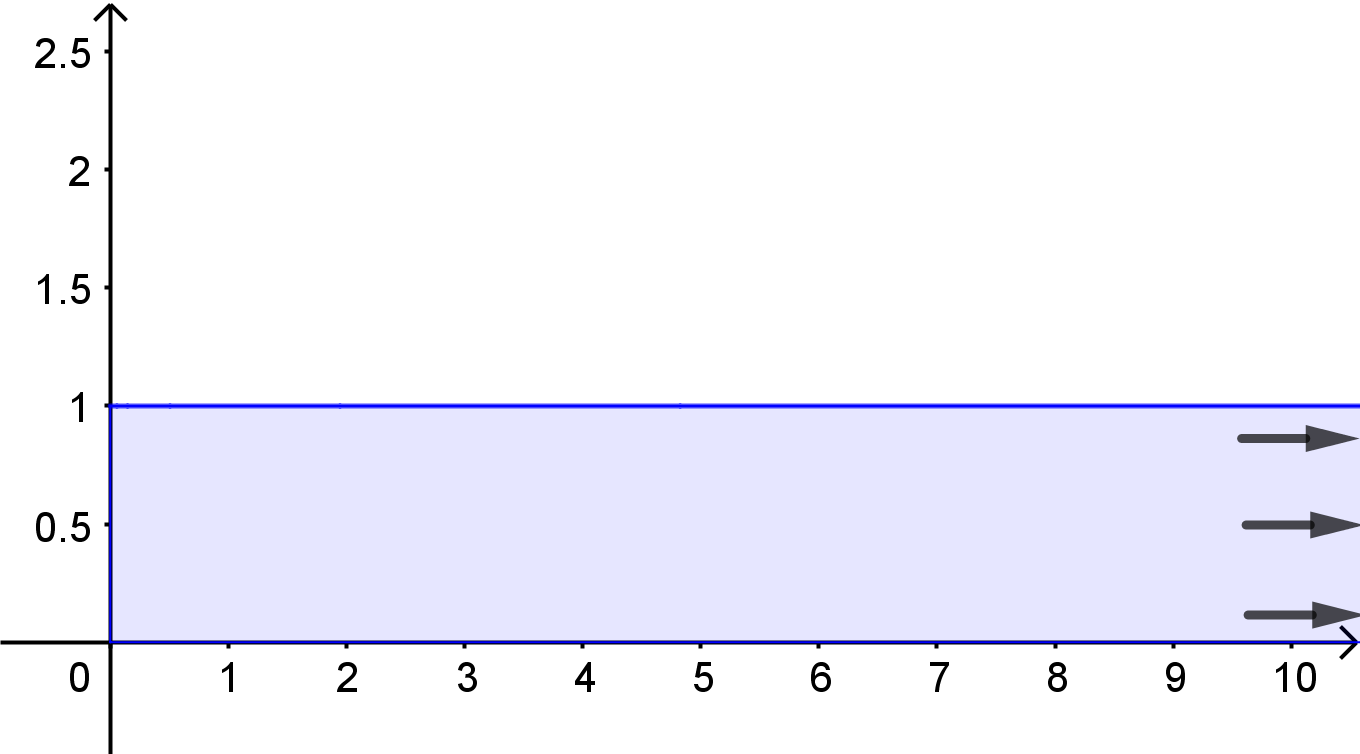
\includegraphics[width=5cm]{img/ej8.png}
            \end{center}
            Así que la integral iterada a resolver es
            \[
                \int_{0}^{\infty}{
                    \int_{0}^{1}{
                        xye^{-(x^2+y^2)}
                    \,dy}
                \,dx}
            \]
            Sustituimos ese infinito con una nueva variable $t$ y hacemos que
            ésta tienda hacia infinito
            \begin{align*}
                \lim_{t\to\infty}{
                    \int_{0}^{t}{
                        \int_{0}^{1}{
                            xye^{-(x^2+y^2)}
                        \,dy}
                    \,dx}
                }
                &=\lim_{t\to\infty}{
                    \int_{0}^{t}{
                        x\left[-\frac{1}{2}e^{-(x^2-y^2)}\right]_0^1
                    \,dx}
                }\\[.3cm]
                &=-\frac{1}{2}\lim_{t\to\infty}{
                    \int_{0}^{t}{
                        x\left[e^{-(x^2+1)}-e^{-x^2}\right]
                    \,dx}
                }\\[.3cm]
                &=-\frac{1}{2}\lim_{t\to\infty}{
                    \int_{0}^{t}{
                        xe^{-x^2}\left[e^{-1}-1\right]
                    \,dx}
                }\\[.3cm]
                &=-\frac{e^{-1}-1}{2}\lim_{t\to\infty}{
                    -\frac{1}{2}\left[-\frac{1}{2}e^{-x^2}\right]_{0}^{t}
                }\\[.3cm]
                &=\frac{e^{-1}-1}{4}\lim_{t\to\infty}{
                    \left(e^{-t^2}-1\right)
                }
            \end{align*}
            Simplificamos la expresión $\frac{e^{-1}-1}{4}=\frac{1-e}{4e}$ y al
            calcular el límite $e^{-t^2}\to 0$ por lo que el límite es
            $-1$ y el resultado de la integral es $\displaystyle\frac{e-1}{4e}$
        }
    \end{enumerate}
\end{document}
